% Chapter Template

\chapter{Estado del Arte} % Main chapter title

\label{Chapter2} % Change X to a consecutive number; for referencing this chapter elsewhere, use \ref{ChapterX}

%----------------------------------------------------------------------------------------
%	SECTION 1
%----------------------------------------------------------------------------------------

\section{An\'alisis de im\'agenes de la retina}

El an\'alisis de im\'agenes de la retina es de gran importancia para la detecci\'on de enfermedades del ojo.
El avance tecnol\'ogico permiti\'o obtener im\'agenes de la retina con mayor calidad, lo que beneficia la detecci\'on precoz de enfermedades con mayor precisi\'on, favoreciendo la disminuci\'on del porcentaje de personas con ceguera debido a enfermedades sistemicas o retinales. 

%-----------------------------------
%	SUBSECTION 1
%-----------------------------------
\subsection{Introducci\'on}

La retina es un tejido en capas que recubre el interior del ojo, permitiendo la conversión de la luz entrante en señales neuronales adecuadas para su posterior procesamiento por parte de la corteza visual del cerebro. La misma está sostenida por el epitelio pigmentario retinal, la coroide y la esclera.

La estructura anatómica del ojo se compone básicamente por la córnea (transparente), la esclera (normalmente blanca), el iris (que da color al ojo) y la pupila. Todas estas partes son visibles desde el exterior, y son las responsables de permitir la visión: un rayo de luz pasa a través de la córnea, que enfoca parcialmente la imagen, luego pasa por la cámara anterior, la pupila (que hace las veces de lente y enfoca aún más la imagen), la vítrea y por último es enfocado en la retina.

VA LA IMAGEN DEL OJO CON SUS PARTES


Actualmente existen diversas \'areas de investigación activas en lo que respecta a la imagenología de la retina. Algunas de las \'areas se centran en la b\'usqueda de herramientas t\'ecnicas rentables, f\'aciles de usar y portables. Por otro lado CONSULTAR IMAGENES FUNCIONALES. Otra \'area (Adaptive Optics) se encarga de la utilizaci\'on de lentes para corregir las fallas de frente de onda de la luz reflejada desde la retina, permitiendo la obtenci\'on de celulas individuales o estructuras celulares.
Longer Wavelength OCT Imaging realiza investigaciones para el desarrollo de los l\'aseres de baja coherencia de c\'odigo de barrido con longitudes de ondas centrales mayores. Algunos de estos prototipos ya son capaces de resolver los detalles en la coroides y la l\'amina cribosa.






%-----------------------------------
%	SUBSECTION 2
%-----------------------------------

\subsection{Fotograf\'ias de fondo de ojo}


Existen diversas formas de poder observar y analizar la anatom\'ia del ojo, a trav\'es de im\'agenes m\'edicas. 
Una de las modalidades de imagen m\'edica que permite explorar el interior del ojo es la de la imagen de fondo de ojo. La misma consiste en  una representaci\'on 2D del tejido retinal semitransparente 3D, proyectado en el plano de obtenci\'on de la imagen, que se obtiene usando la luz reflejada en el tejido.

Para realizar la captura del fondo de ojo, se dilata la pupila con f\'armacos que se depositan en forma de gotas en la superficie ocular; as\'i, el oftalm\'ologo puede ver con facilidad el interior del globo ocular con un aparato que se llama oftalmoscopio. El oftalmoscopio consiste en un aparato formado por una serie de espejos y cristales que alumbran la retina del ojo sin que la luz se refleje. Si no fuese por el oftalmoscopio la luz provocar\'ia destellos y no se podría ver el fondo de ojo de manera correcta, algo parecido a lo que sucede cuando el flash de una cámara de fotos saca los ojos en color rojo. Esta modalidad no es invasiva, y su costo es menor a la angiografía y la OCT dado que la c\'amara que se necesita para capturar la imagen del ojo es una c\'amara digital convencional.
Adem\'as de facilitar la detecci\'on de enfermedades oculares, las im\'agenes de fondo de ojo permiten detectar tres tipos de lesiones oculares. 


\begin{figure}[h]
%\centering
\minipage{0.32\textwidth}
	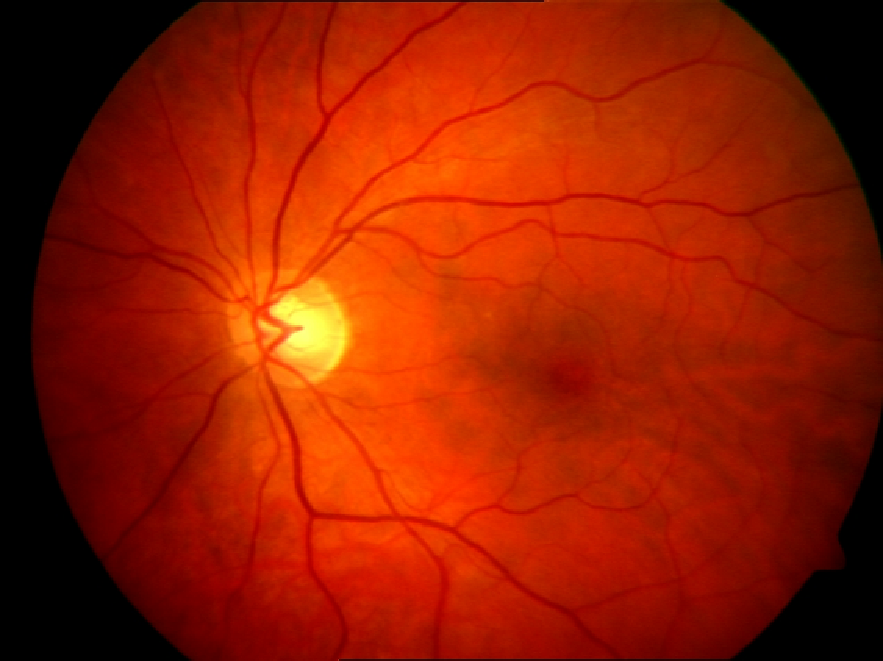
\includegraphics[width=\linewidth]{Figures/images}
	\caption[HRF]{HRF (Degeneración macular).}\label{fig:HRF}
\endminipage\hfill
%\decoRule
%\caption[HRF]{HRF (Degeneración macular).}
\minipage{0.32\textwidth}
	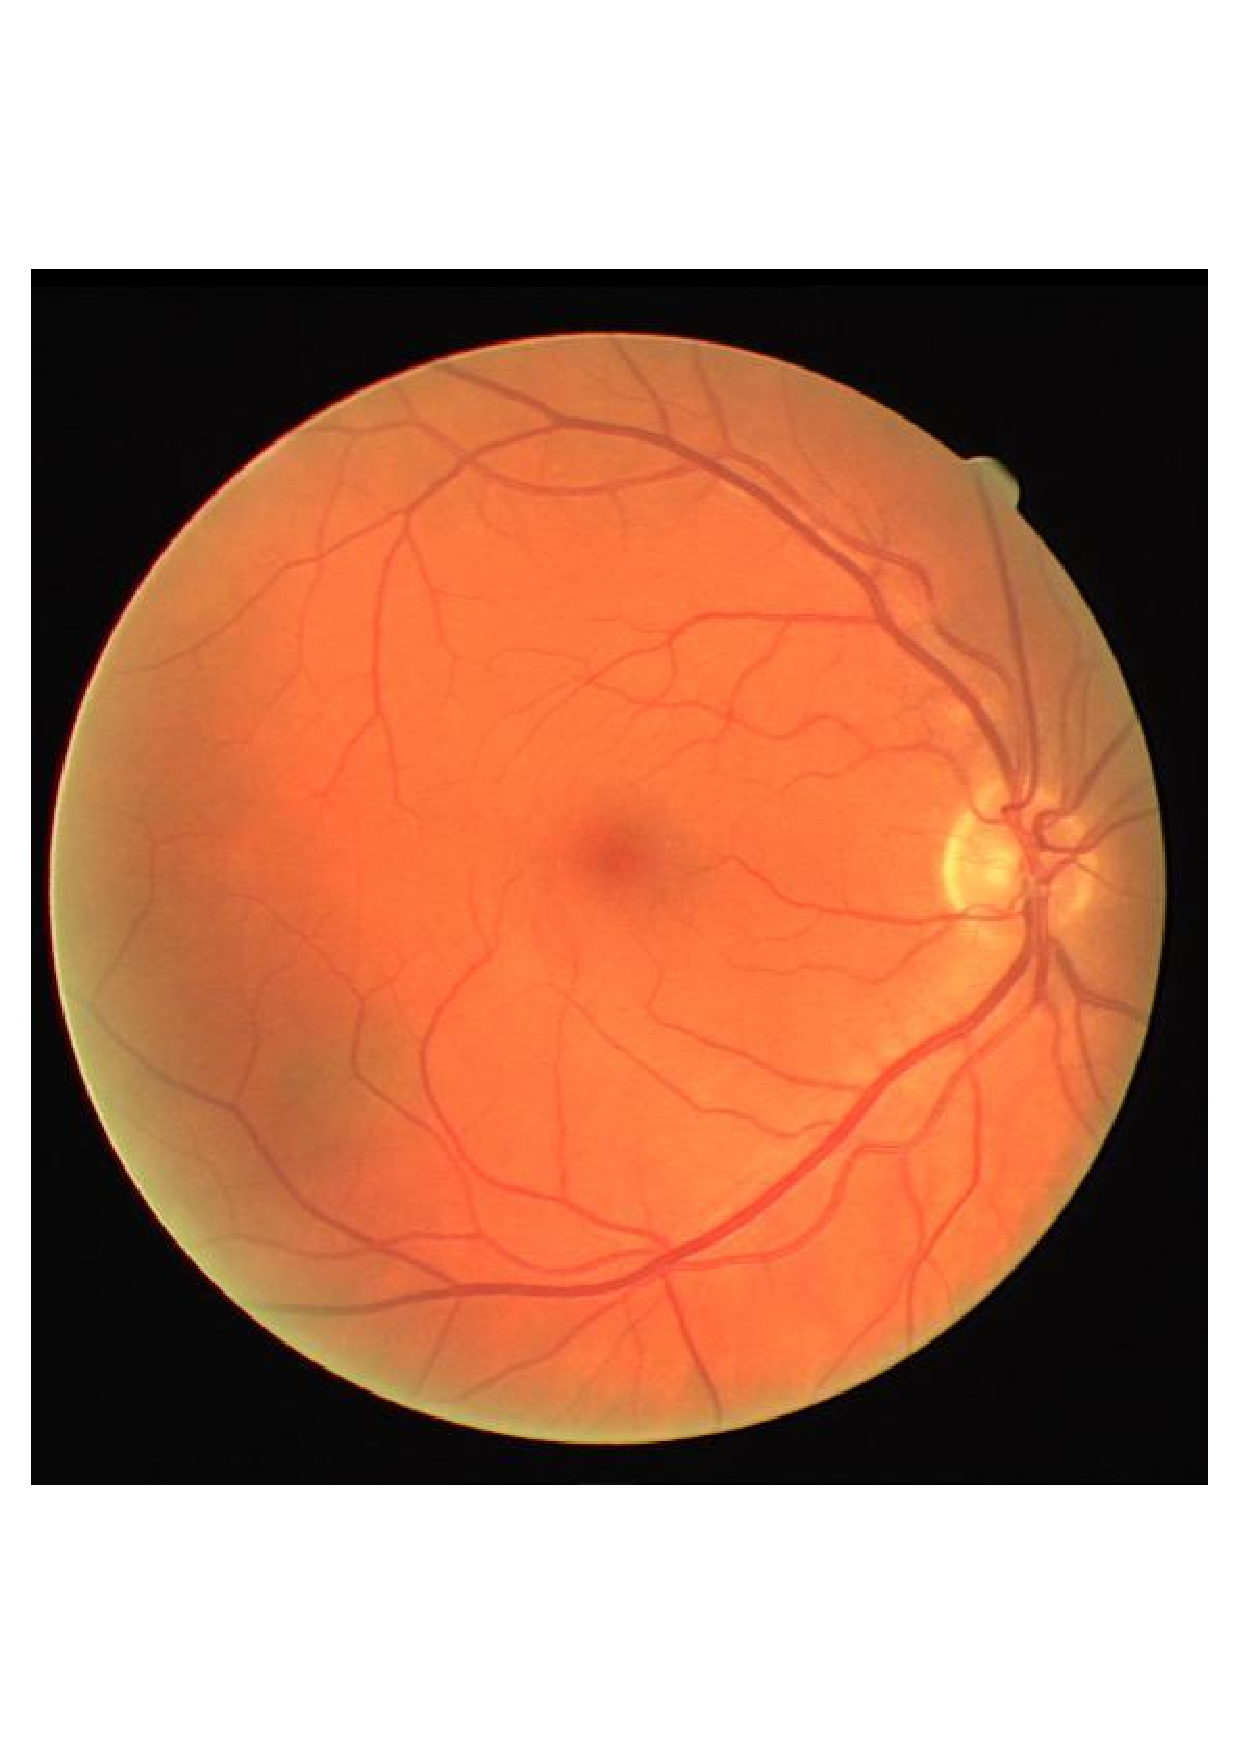
\includegraphics[width=\linewidth]{Figures/images1}
	\caption[ARIA]{ARIA (Degeneración macular).}\label{fig:ARIA}
\endminipage\hfill
\minipage{0.32\textwidth}
	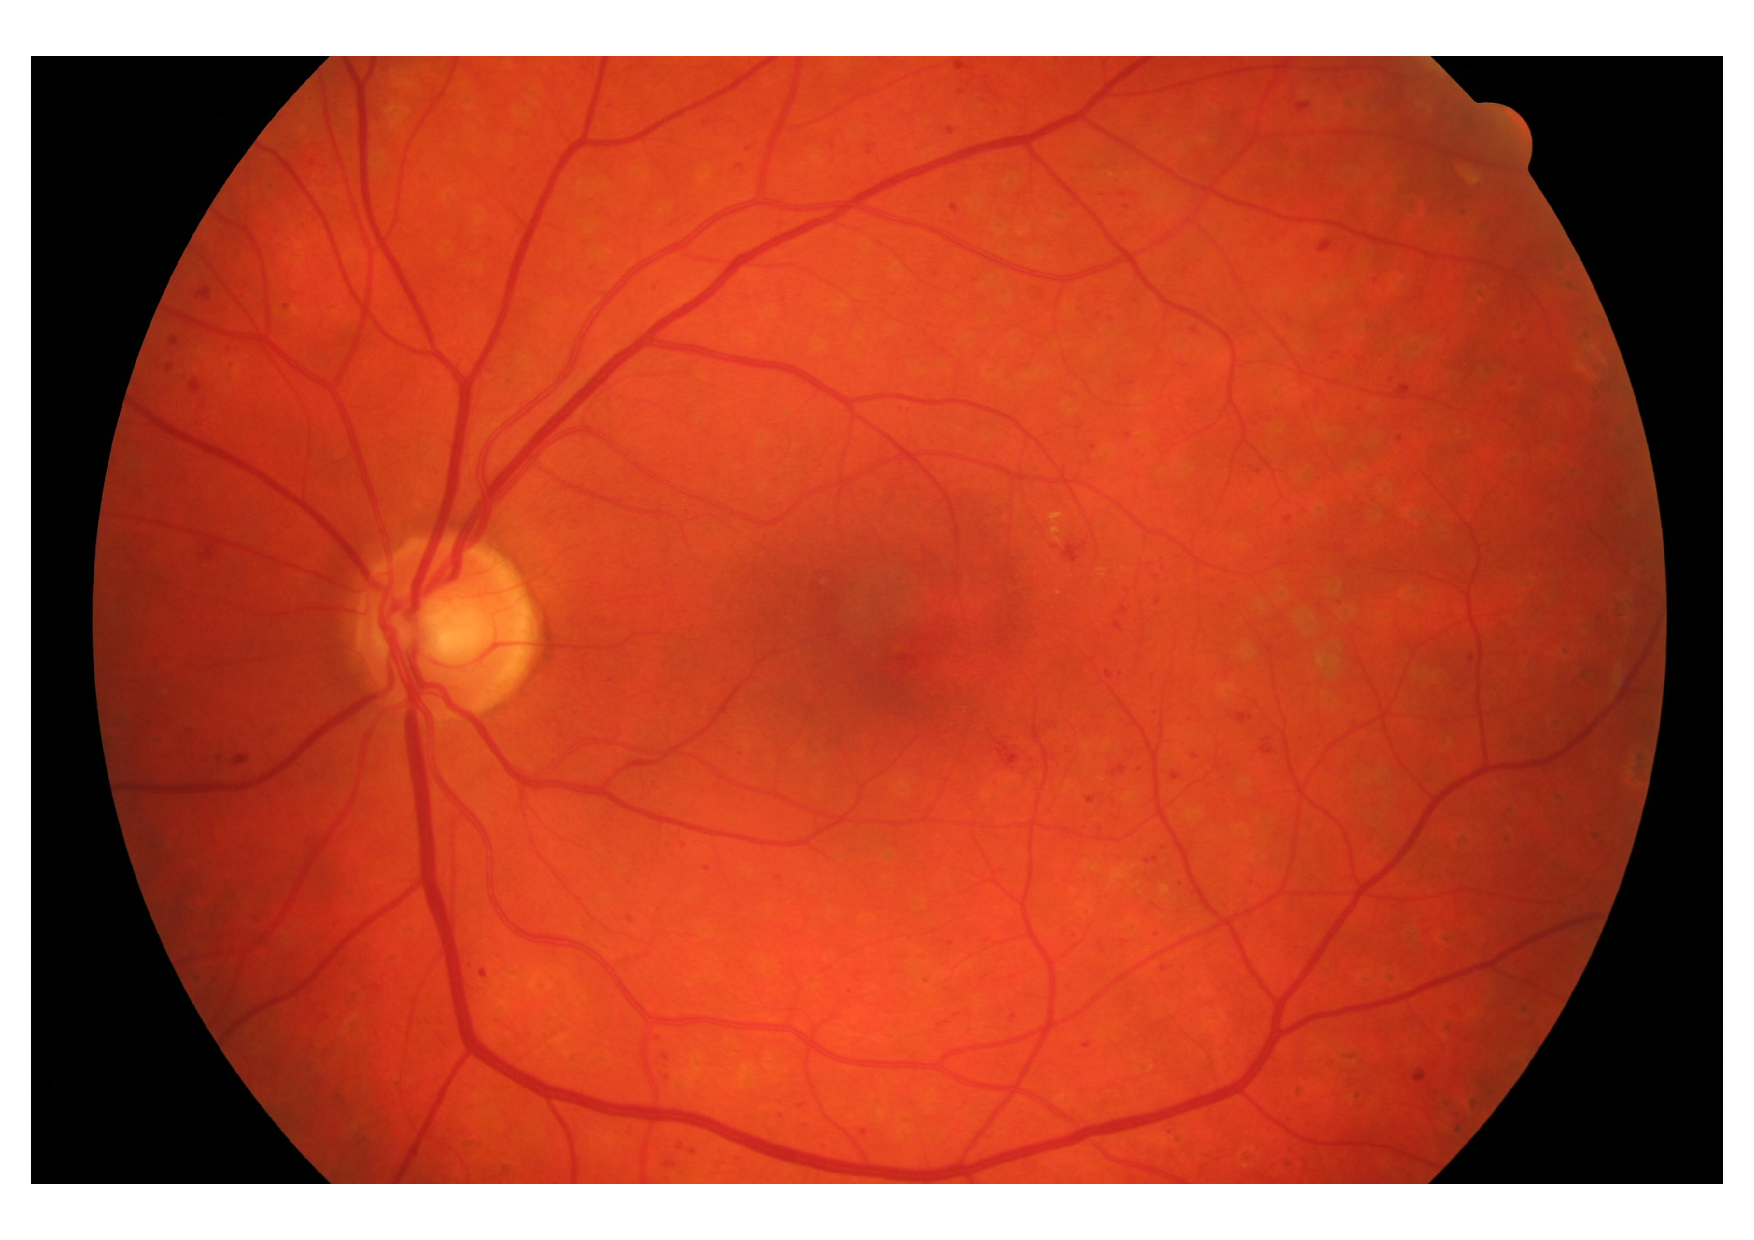
\includegraphics[width=\linewidth]{Figures/images2}
	\caption[HRF]{HRF (Degeneración macular).}\label{fig:HRF}
\endminipage\hfill

%\label{fig:Electron}
\end{figure}


%-----------------------------------
%	SUBSECTION 3
%-----------------------------------

\subsection{Herramientas computacionales para an\'alisis de fotograf\'ias de fondo de ojo}
Morbi rutrum odio eget arcu adipiscing sodales. Aenean et purus a est pulvinar pellentesque. Cras in elit neque, quis varius elit. Phasellus fringilla, nibh eu tempus venenatis, dolor elit posuere quam, quis adipiscing urna leo nec orci. Sed nec nulla auctor odio aliquet consequat. Ut nec nulla in ante ullamcorper aliquam at sed dolor. Phasellus fermentum magna in augue gravida cursus. Cras sed pretium lorem. Pellentesque eget ornare odio. Proin accumsan, massa viverra cursus pharetra, ipsum nisi lobortis velit, a malesuada dolor lorem eu neque.

%----------------------------------------------------------------------------------------
%	SECTION 2
%----------------------------------------------------------------------------------------

\section{Segmentaci\'on de vasos sangu\'ineos en im\'agenes de fondo de ojo}

Sed ullamcorper quam eu nisl interdum at interdum enim egestas. Aliquam placerat justo sed lectus lobortis ut porta nisl porttitor. Vestibulum mi dolor, lacinia molestie gravida at, tempus vitae ligula. Donec eget quam sapien, in viverra eros. Donec pellentesque justo a massa fringilla non vestibulum metus vestibulum. Vestibulum in orci quis felis tempor lacinia. Vivamus ornare ultrices facilisis. Ut hendrerit volutpat vulputate. Morbi condimentum venenatis augue, id porta ipsum vulputate in. Curabitur luctus tempus justo. Vestibulum risus lectus, adipiscing nec condimentum quis, condimentum nec nisl. Aliquam dictum sagittis velit sed iaculis. Morbi tristique augue sit amet nulla pulvinar id facilisis ligula mollis. Nam elit libero, tincidunt ut aliquam at, molestie in quam. Aenean rhoncus vehicula hendrerit.

%-----------------------------------
%	SUBSECTION 1
%-----------------------------------

\subsection{Necesidad}
Morbi rutrum odio eget arcu adipiscing sodales. Aenean et purus a est pulvinar pellentesque. Cras in elit neque, quis varius elit. Phasellus fringilla, nibh eu tempus venenatis, dolor elit posuere quam, quis adipiscing urna leo nec orci. Sed nec nulla auctor odio aliquet consequat. Ut nec nulla in ante ullamcorper aliquam at sed dolor. Phasellus fermentum magna in augue gravida cursus. Cras sed pretium lorem. Pellentesque eget ornare odio. Proin accumsan, massa viverra cursus pharetra, ipsum nisi lobortis velit, a malesuada dolor lorem eu neque.

%-----------------------------------
%	SUBSECTION 2
%-----------------------------------

\subsection{M\'etodos existentes}
Morbi rutrum odio eget arcu adipiscing sodales. Aenean et purus a est pulvinar pellentesque. Cras in elit neque, quis varius elit. Phasellus fringilla, nibh eu tempus venenatis, dolor elit posuere quam, quis adipiscing urna leo nec orci. Sed nec nulla auctor odio aliquet consequat. Ut nec nulla in ante ullamcorper aliquam at sed dolor. Phasellus fermentum magna in augue gravida cursus. Cras sed pretium lorem. Pellentesque eget ornare odio. Proin accumsan, massa viverra cursus pharetra, ipsum nisi lobortis velit, a malesuada dolor lorem eu neque.
